
%% bare_jrnl.tex
%% V1.4b
%% 2015/08/26
%% by Michael Shell
%% see http://www.michaelshell.org/
%% for current contact information.
%%
%% This is a skeleton file demonstrating the use of IEEEtran.cls
%% (requires IEEEtran.cls version 1.8b or later) with an IEEE
%% journal paper.
%%
%% Support sites:
%% http://www.michaelshell.org/tex/ieeetran/
%% http://www.ctan.org/pkg/ieeetran
%% and
%% http://www.ieee.org/

%%*************************************************************************
%% Legal Notice:
%% This code is offered as-is without any warranty either expressed or
%% implied; without even the implied warranty of MERCHANTABILITY or
%% FITNESS FOR A PARTICULAR PURPOSE! 
%% User assumes all risk.
%% In no event shall the IEEE or any contributor to this code be liable for
%% any damages or losses, including, but not limited to, incidental,
%% consequential, or any other damages, resulting from the use or misuse
%% of any information contained here.
%%
%% All comments are the opinions of their respective authors and are not
%% necessarily endorsed by the IEEE.
%%
%% This work is distributed under the LaTeX Project Public License (LPPL)
%% ( http://www.latex-project.org/ ) version 1.3, and may be freely used,
%% distributed and modified. A copy of the LPPL, version 1.3, is included
%% in the base LaTeX documentation of all distributions of LaTeX released
%% 2003/12/01 or later.
%% Retain all contribution notices and credits.
%% ** Modified files should be clearly indicated as such, including  **
%% ** renaming them and changing author support contact information. **
%%*************************************************************************


% *** Authors should verify (and, if needed, correct) their LaTeX system  ***
% *** with the testflow diagnostic prior to trusting their LaTeX platform ***
% *** with production work. The IEEE's font choices and paper sizes can   ***
% *** trigger bugs that do not appear when using other class files.       ***                          ***
% The testflow support page is at:
% http://www.michaelshell.org/tex/testflow/



\documentclass[journal]{IEEEtran}
%
% If IEEEtran.cls has not been installed into the LaTeX system files,
% manually specify the path to it like:
% \documentclass[journal]{../sty/IEEEtran}





% Some very useful LaTeX packages include:
% (uncomment the ones you want to load)


% *** MISC UTILITY PACKAGES ***
%
%\usepackage{ifpdf}
% Heiko Oberdiek's ifpdf.sty is very useful if you need conditional
% compilation based on whether the output is pdf or dvi.
% usage:
% \ifpdf
%   % pdf code
% \else
%   % dvi code
% \fi
% The latest version of ifpdf.sty can be obtained from:
% http://www.ctan.org/pkg/ifpdf
% Also, note that IEEEtran.cls V1.7 and later provides a builtin
% \ifCLASSINFOpdf conditional that works the same way.
% When switching from latex to pdflatex and vice-versa, the compiler may
% have to be run twice to clear warning/error messages.






% *** CITATION PACKAGES ***
%
%\usepackage{cite}
% cite.sty was written by Donald Arseneau
% V1.6 and later of IEEEtran pre-defines the format of the cite.sty package
% \cite{} output to follow that of the IEEE. Loading the cite package will
% result in citation numbers being automatically sorted and properly
% "compressed/ranged". e.g., [1], [9], [2], [7], [5], [6] without using
% cite.sty will become [1], [2], [5]--[7], [9] using cite.sty. cite.sty's
% \cite will automatically add leading space, if needed. Use cite.sty's
% noadjust option (cite.sty V3.8 and later) if you want to turn this off
% such as if a citation ever needs to be enclosed in parenthesis.
% cite.sty is already installed on most LaTeX systems. Be sure and use
% version 5.0 (2009-03-20) and later if using hyperref.sty.
% The latest version can be obtained at:
% http://www.ctan.org/pkg/cite
% The documentation is contained in the cite.sty file itself.


\usepackage{graphicx}
\usepackage{subfigure}
\usepackage{booktabs}
\usepackage[noadjust]{cite}
\renewcommand{\citepunct}{,\penalty\citepunctpenalty\,}
\renewcommand{\citedash}{--}
\usepackage{hyperref}

% *** GRAPHICS RELATED PACKAGES ***
%
\ifCLASSINFOpdf
  % \usepackage[pdftex]{graphicx}
  % declare the path(s) where your graphic files are
  % \graphicspath{{../pdf/}{../jpeg/}}
  % and their extensions so you won't have to specify these with
  % every instance of \includegraphics
  % \DeclareGraphicsExtensions{.pdf,.jpeg,.png}
\else
  % or other class option (dvipsone, dvipdf, if not using dvips). graphicx
  % will default to the driver specified in the system graphics.cfg if no
  % driver is specified.
  % \usepackage[dvips]{graphicx}
  % declare the path(s) where your graphic files are
  % \graphicspath{{../eps/}}
  % and their extensions so you won't have to specify these with
  % every instance of \includegraphics
  % \DeclareGraphicsExtensions{.eps}
\fi
% graphicx was written by David Carlisle and Sebastian Rahtz. It is
% required if you want graphics, photos, etc. graphicx.sty is already
% installed on most LaTeX systems. The latest version and documentation
% can be obtained at: 
% http://www.ctan.org/pkg/graphicx
% Another good source of documentation is "Using Imported Graphics in
% LaTeX2e" by Keith Reckdahl which can be found at:
% http://www.ctan.org/pkg/epslatex
%
% latex, and pdflatex in dvi mode, support graphics in encapsulated
% postscript (.eps) format. pdflatex in pdf mode supports graphics
% in .pdf, .jpeg, .png and .mps (metapost) formats. Users should ensure
% that all non-photo figures use a vector format (.eps, .pdf, .mps) and
% not a bitmapped formats (.jpeg, .png). The IEEE frowns on bitmapped formats
% which can result in "jaggedy"/blurry rendering of lines and letters as
% well as large increases in file sizes.
%
% You can find documentation about the pdfTeX application at:
% http://www.tug.org/applications/pdftex





% *** MATH PACKAGES ***
%
\usepackage{amsmath}
% A popular package from the American Mathematical Society that provides
% many useful and powerful commands for dealing with mathematics.
%
% Note that the amsmath package sets \interdisplaylinepenalty to 10000
% thus preventing page breaks from occurring within multiline equations. Use:
%\interdisplaylinepenalty=2500
% after loading amsmath to restore such page breaks as IEEEtran.cls normally
% does. amsmath.sty is already installed on most LaTeX systems. The latest
% version and documentation can be obtained at:
% http://www.ctan.org/pkg/amsmath





% *** SPECIALIZED LIST PACKAGES ***
%
%\usepackage{algorithmic}
% algorithmic.sty was written by Peter Williams and Rogerio Brito.
% This package provides an algorithmic environment fo describing algorithms.
% You can use the algorithmic environment in-text or within a figure
% environment to provide for a floating algorithm. Do NOT use the algorithm
% floating environment provided by algorithm.sty (by the same authors) or
% algorithm2e.sty (by Christophe Fiorio) as the IEEE does not use dedicated
% algorithm float types and packages that provide these will not provide
% correct IEEE style captions. The latest version and documentation of
% algorithmic.sty can be obtained at:
% http://www.ctan.org/pkg/algorithms
% Also of interest may be the (relatively newer and more customizable)
% algorithmicx.sty package by Szasz Janos:
% http://www.ctan.org/pkg/algorithmicx




% *** ALIGNMENT PACKAGES ***
%
%\usepackage{array}
% Frank Mittelbach's and David Carlisle's array.sty patches and improves
% the standard LaTeX2e array and tabular environments to provide better
% appearance and additional user controls. As the default LaTeX2e table
% generation code is lacking to the point of almost being broken with
% respect to the quality of the end results, all users are strongly
% advised to use an enhanced (at the very least that provided by array.sty)
% set of table tools. array.sty is already installed on most systems. The
% latest version and documentation can be obtained at:
% http://www.ctan.org/pkg/array


% IEEEtran contains the IEEEeqnarray family of commands that can be used to
% generate multiline equations as well as matrices, tables, etc., of high
% quality.




% *** SUBFIGURE PACKAGES ***
%\ifCLASSOPTIONcompsoc
%  \usepackage[caption=false,font=normalsize,labelfont=sf,textfont=sf]{subfig}
%\else
%  \usepackage[caption=false,font=footnotesize]{subfig}
%\fi
% subfig.sty, written by Steven Douglas Cochran, is the modern replacement
% for subfigure.sty, the latter of which is no longer maintained and is
% incompatible with some LaTeX packages including fixltx2e. However,
% subfig.sty requires and automatically loads Axel Sommerfeldt's caption.sty
% which will override IEEEtran.cls' handling of captions and this will result
% in non-IEEE style figure/table captions. To prevent this problem, be sure
% and invoke subfig.sty's "caption=false" package option (available since
% subfig.sty version 1.3, 2005/06/28) as this is will preserve IEEEtran.cls
% handling of captions.
% Note that the Computer Society format requires a larger sans serif font
% than the serif footnote size font used in traditional IEEE formatting
% and thus the need to invoke different subfig.sty package options depending
% on whether compsoc mode has been enabled.
%
% The latest version and documentation of subfig.sty can be obtained at:
% http://www.ctan.org/pkg/subfig




% *** FLOAT PACKAGES ***
%
%\usepackage{fixltx2e}
% fixltx2e, the successor to the earlier fix2col.sty, was written by
% Frank Mittelbach and David Carlisle. This package corrects a few problems
% in the LaTeX2e kernel, the most notable of which is that in current
% LaTeX2e releases, the ordering of single and double column floats is not
% guaranteed to be preserved. Thus, an unpatched LaTeX2e can allow a
% single column figure to be placed prior to an earlier double column
% figure.
% Be aware that LaTeX2e kernels dated 2015 and later have fixltx2e.sty's
% corrections already built into the system in which case a warning will
% be issued if an attempt is made to load fixltx2e.sty as it is no longer
% needed.
% The latest version and documentation can be found at:
% http://www.ctan.org/pkg/fixltx2e


%\usepackage{stfloats}
% stfloats.sty was written by Sigitas Tolusis. This package gives LaTeX2e
% the ability to do double column floats at the bottom of the page as well
% as the top. (e.g., "\begin{figure*}[!b]" is not normally possible in
% LaTeX2e). It also provides a command:
%\fnbelowfloat
% to enable the placement of footnotes below bottom floats (the standard
% LaTeX2e kernel puts them above bottom floats). This is an invasive package
% which rewrites many portions of the LaTeX2e float routines. It may not work
% with other packages that modify the LaTeX2e float routines. The latest
% version and documentation can be obtained at:
% http://www.ctan.org/pkg/stfloats
% Do not use the stfloats baselinefloat ability as the IEEE does not allow
% \baselineskip to stretch. Authors submitting work to the IEEE should note
% that the IEEE rarely uses double column equations and that authors should try
% to avoid such use. Do not be tempted to use the cuted.sty or midfloat.sty
% packages (also by Sigitas Tolusis) as the IEEE does not format its papers in
% such ways.
% Do not attempt to use stfloats with fixltx2e as they are incompatible.
% Instead, use Morten Hogholm'a dblfloatfix which combines the features
% of both fixltx2e and stfloats:
%
% \usepackage{dblfloatfix}
% The latest version can be found at:
% http://www.ctan.org/pkg/dblfloatfix




%\ifCLASSOPTIONcaptionsoff
%  \usepackage[nomarkers]{endfloat}
% \let\MYoriglatexcaption\caption
% \renewcommand{\caption}[2][\relax]{\MYoriglatexcaption[#2]{#2}}
%\fi
% endfloat.sty was written by James Darrell McCauley, Jeff Goldberg and 
% Axel Sommerfeldt. This package may be useful when used in conjunction with 
% IEEEtran.cls'  captionsoff option. Some IEEE journals/societies require that
% submissions have lists of figures/tables at the end of the paper and that
% figures/tables without any captions are placed on a page by themselves at
% the end of the document. If needed, the draftcls IEEEtran class option or
% \CLASSINPUTbaselinestretch interface can be used to increase the line
% spacing as well. Be sure and use the nomarkers option of endfloat to
% prevent endfloat from "marking" where the figures would have been placed
% in the text. The two hack lines of code above are a slight modification of
% that suggested by in the endfloat docs (section 8.4.1) to ensure that
% the full captions always appear in the list of figures/tables - even if
% the user used the short optional argument of \caption[]{}.
% IEEE papers do not typically make use of \caption[]'s optional argument,
% so this should not be an issue. A similar trick can be used to disable
% captions of packages such as subfig.sty that lack options to turn off
% the subcaptions:
% For subfig.sty:
% \let\MYorigsubfloat\subfloat
% \renewcommand{\subfloat}[2][\relax]{\MYorigsubfloat[]{#2}}
% However, the above trick will not work if both optional arguments of
% the \subfloat command are used. Furthermore, there needs to be a
% description of each subfigure *somewhere* and endfloat does not add
% subfigure captions to its list of figures. Thus, the best approach is to
% avoid the use of subfigure captions (many IEEE journals avoid them anyway)
% and instead reference/explain all the subfigures within the main caption.
% The latest version of endfloat.sty and its documentation can obtained at:
% http://www.ctan.org/pkg/endfloat
%
% The IEEEtran \ifCLASSOPTIONcaptionsoff conditional can also be used
% later in the document, say, to conditionally put the References on a 
% page by themselves.




% *** PDF, URL AND HYPERLINK PACKAGES ***
%
%\usepackage{url}
% url.sty was written by Donald Arseneau. It provides better support for
% handling and breaking URLs. url.sty is already installed on most LaTeX
% systems. The latest version and documentation can be obtained at:
% http://www.ctan.org/pkg/url
% Basically, \url{my_url_here}.




% *** Do not adjust lengths that control margins, column widths, etc. ***
% *** Do not use packages that alter fonts (such as pslatex).         ***
% There should be no need to do such things with IEEEtran.cls V1.6 and later.
% (Unless specifically asked to do so by the journal or conference you plan
% to submit to, of course. )


% correct bad hyphenation here
\hyphenation{op-tical net-works semi-conduc-tor}


\begin{document}
%
% paper title
% Titles are generally capitalized except for words such as a, an, and, as,
% at, but, by, for, in, nor, of, on, or, the, to and up, which are usually
% not capitalized unless they are the first or last word of the title.
% Linebreaks \\ can be used within to get better formatting as desired.
% Do not put math or special symbols in the title.
\title{Attention-based LSTM: A Machine Leanring Approach for Automatic Sleep Stages Classification}
%
%
% author names and IEEE memberships
% note positions of commas and nonbreaking spaces ( ~ ) LaTeX will not break
% a structure at a ~ so this keeps an author's name from being broken across
% two lines.
% use \thanks{} to gain access to the first footnote area
% a separate \thanks must be used for each paragraph as LaTeX2e's \thanks
% was not built to handle multiple paragraphs
%

\author{Junbin~Huang$^{1}$,
        Pengcheng~Wang$^{2}$,
        Cong~Xie$^{3}$,
        Zehan~Zhang$^{4}$,
        Donglai~Sun$^{5}$\\
        \bigskip 
        $^{1,2,3,4,5}$Maxtropy Technology, Shanghai 201199, China\\
        \textit{\{huangjunbin,wangpengcheng,xiecong,zhangzehan,sundonglai\}@maxtropy.com}
        % <-this % stops a space
%\thanks{M. Shell was with the Department
%of Electrical and Computer Engineering, Georgia Institute of Technology, Atlanta,
%GA, 30332 USA e-mail: (see http://www.michaelshell.org/contact.html).}% <-this % stops a space
%\thanks{J. Doe and J. Doe are with Anonymous University.}% <-this % stops a space
%\thanks{Manuscript received April 19, 2005; revised August 26, 2015.}
}

% note the % following the last \IEEEmembership and also \thanks - 
% these prevent an unwanted space from occurring between the last author name
% and the end of the author line. i.e., if you had this:
% 
% \author{....lastname \thanks{...} \thanks{...} }
%                     ^------------^------------^----Do not want these spaces!
%
% a space would be appended to the last name and could cause every name on that
% line to be shifted left slightly. This is one of those "LaTeX things". For
% instance, "\textbf{A} \textbf{B}" will typeset as "A B" not "AB". To get
% "AB" then you have to do: "\textbf{A}\textbf{B}"
% \thanks is no different in this regard, so shield the last } of each \thanks
% that ends a line with a % and do not let a space in before the next \thanks.
% Spaces after \IEEEmembership other than the last one are OK (and needed) as
% you are supposed to have spaces between the names. For what it is worth,
% this is a minor point as most people would not even notice if the said evil
% space somehow managed to creep in.



% The paper headers
\markboth{Submitted Paper for IEEE Transactions on Affective Computing}%
{Shell \MakeLowercase{\textit{et al.}}: Bare Demo of IEEEtran.cls for IEEE Journals}
% The only time the second header will appear is for the odd numbered pages
% after the title page when using the twoside option.
% 
% *** Note that you probably will NOT want to include the author's ***
% *** name in the headers of peer review papers.                   ***
% You can use \ifCLASSOPTIONpeerreview for conditional compilation here if
% you desire.




% If you want to put a publisher's ID mark on the page you can do it like
% this:
%\IEEEpubid{0000--0000/00\$00.00~\copyright~2015 IEEE}
% Remember, if you use this you must call \IEEEpubidadjcol in the second
% column for its text to clear the IEEEpubid mark.



% use for special paper notices
%\IEEEspecialpapernotice{(Invited Paper)}




% make the title area
\maketitle

% As a general rule, do not put math, special symbols or citations
% in the abstract or keywords.
\begin{abstract}
The abstract goes here.
\end{abstract}

% Note that keywords are not normally used for peerreview papers.
\begin{IEEEkeywords}
IEEE, IEEEtran, journal, \LaTeX, paper, template.
\end{IEEEkeywords}






% For peer review papers, you can put extra information on the cover
% page as needed:
% \ifCLASSOPTIONpeerreview
% \begin{center} \bfseries EDICS Category: 3-BBND \end{center}
% \fi
%
% For peerreview papers, this IEEEtran command inserts a page break and
% creates the second title. It will be ignored for other modes.
\IEEEpeerreviewmaketitle



\section{Introduction}
% The very first letter is a 2 line initial drop letter followed
% by the rest of the first word in caps.
% 
% form to use if the first word consists of a single letter:
% \IEEEPARstart{A}{demo} file is ....
% 
% form to use if you need the single drop letter followed by
% normal text (unknown if ever used by the IEEE):
% \IEEEPARstart{A}{}demo file is ....
% 
% Some journals put the first two words in caps:
% \IEEEPARstart{T}{his demo} file is ....
% 
% Here we have the typical use of a "T" for an initial drop letter
% and "HIS" in caps to complete the first word.
\IEEEPARstart{T}{his} demo file is intended to serve as a ``starter file''
for IEEE journal papers produced under \LaTeX\ using
IEEEtran.cls version 1.8b and  later.
% You must have at least 2 lines in the paragraph with the drop letter
% (should never be an issue)
I wish you the best of success.

Such a method has been applied by several groups 

Most of the proposed sleep stage classification models belong to a family of model selection, with a certain feature set for the PSG data and a general model like Support Vector Machine or Random Forest.

The potential issue with this feature selection approach is that the features selected need to compress all the necessary information of the specific bio-information signals.

\subsection{Subsection Heading Here}
Subsection text here.

% needed in second column of first page if using \IEEEpubid
%\IEEEpubidadjcol

\subsubsection{Subsubsection Heading Here}
Subsubsection text here.


% An example of a floating figure using the graphicx package.
% Note that \label must occur AFTER (or within) \caption.
% For figures, \caption should occur after the \includegraphics.
% Note that IEEEtran v1.7 and later has special internal code that
% is designed to preserve the operation of \label within \caption
% even when the captionsoff option is in effect. However, because
% of issues like this, it may be the safest practice to put all your
% \label just after \caption rather than within \caption{}.
%
% Reminder: the "draftcls" or "draftclsnofoot", not "draft", class
% option should be used if it is desired that the figures are to be
% displayed while in draft mode.
%
%\begin{figure}[!t]
%\centering
%\includegraphics[width=2.5in]{myfigure}
% where an .eps filename suffix will be assumed under latex, 
% and a .pdf suffix will be assumed for pdflatex; or what has been declared
% via \DeclareGraphicsExtensions.
%\caption{Simulation results for the network.}
%\label{fig_sim}
%\end{figure}

% Note that the IEEE typically puts floats only at the top, even when this
% results in a large percentage of a column being occupied by floats.


% An example of a double column floating figure using two subfigures.
% (The subfig.sty package must be loaded for this to work.)
% The subfigure \label commands are set within each subfloat command,
% and the \label for the overall figure must come after \caption.
% \hfil is used as a separator to get equal spacing.
% Watch out that the combined width of all the subfigures on a 
% line do not exceed the text width or a line break will occur.
%
%\begin{figure*}[!t]
%\centering
%\subfloat[Case I]{\includegraphics[width=2.5in]{box}%
%\label{fig_first_case}}
%\hfil
%\subfloat[Case II]{\includegraphics[width=2.5in]{box}%
%\label{fig_second_case}}
%\caption{Simulation results for the network.}
%\label{fig_sim}
%\end{figure*}
%
% Note that often IEEE papers with subfigures do not employ subfigure
% captions (using the optional argument to \subfloat[]), but instead will
% reference/describe all of them (a), (b), etc., within the main caption.
% Be aware that for subfig.sty to generate the (a), (b), etc., subfigure
% labels, the optional argument to \subfloat must be present. If a
% subcaption is not desired, just leave its contents blank,
% e.g., \subfloat[].


% An example of a floating table. Note that, for IEEE style tables, the
% \caption command should come BEFORE the table and, given that table
% captions serve much like titles, are usually capitalized except for words
% such as a, an, and, as, at, but, by, for, in, nor, of, on, or, the, to
% and up, which are usually not capitalized unless they are the first or
% last word of the caption. Table text will default to \footnotesize as
% the IEEE normally uses this smaller font for tables.
% The \label must come after \caption as always.
%
%\begin{table}[!t]
%% increase table row spacing, adjust to taste
%\renewcommand{\arraystretch}{1.3}
% if using array.sty, it might be a good idea to tweak the value of
% \extrarowheight as needed to properly center the text within the cells
%\caption{An Example of a Table}
%\label{table_example}
%\centering
%% Some packages, such as MDW tools, offer better commands for making tables
%% than the plain LaTeX2e tabular which is used here.
%\begin{tabular}{|c||c|}
%\hline
%One & Two\\
%\hline
%Three & Four\\
%\hline
%\end{tabular}
%\end{table}


% Note that the IEEE does not put floats in the very first column
% - or typically anywhere on the first page for that matter. Also,
% in-text middle ("here") positioning is typically not used, but it
% is allowed and encouraged for Computer Society conferences (but
% not Computer Society journals). Most IEEE journals/conferences use
% top floats exclusively. 
% Note that, LaTeX2e, unlike IEEE journals/conferences, places
% footnotes above bottom floats. This can be corrected via the
% \fnbelowfloat command of the stfloats package.


\section{Methods}

\subsection{Attention Mechanism}
Nueral processing mechanisms involving attention have been deeply investigated in Neuroscience and Computational Neuroscience \cite{itti1998model,desimone1995neural}.As the mental activity perfromed by human, attention is definded as an ability of focusing on specific subsets of the received information despite of their position. By applying this mechanism, neural network can learn as what human being can do\cite{zhou2016attention,bahdanau2014neural}.

For time-sequence data, learning a soft alignment between the input and the output improves performance \cite{bahdanau2014neural}. Attention-based model are mainly consiss of the encoder-decoder sequence with fixed length of inner representation. The encoder is used to represent important features of the input sequence with fixed outputs, and the decoder is built to generate the output according to the results of the encoder. Both of the encoder and the decoder are comprised of one or more RNN layers \cite{prabhavalkar2017analysis}. An attention layer between the encoder and the decoder helps the system to mining and select profounder relationship between the representation of encoder and the prediction of decoder. By keeping each output of the encoder, training to focus on subsets of them selectively and then re-link them to the output of decoder, the attention layer frees the model from the loss of compressing features into a fixed length vector and the training of the network will concentrate more on the most important parts \cite{bahdanau2014neural} .

In previously proposed feature-selection-based model, the goal of the sleep stage classifier is to learn and represent the possibility distribution over output prediction $y$ conditioned on the input feature set $X$, i.e. $P(y|X)$ \cite{prabhavalkar2017analysis}.. By combining with the attention model, the RNN model will be able to learn the distribution of each output $y_n$ in condition with the previous epochs of the sleep stage, i.e. $y_{i<n}$, and the input feature stream, $X = {x_1, x_2, X_3, ..., x_m}$:
\begin{equation}
P(y|X) = \prod_n P(y_n|X,y_{i<n})
\end{equation}
With the attention mechanism, the conditional probability in Eq.(1) can be rewrited as:
\begin{equation}
\begin{aligned}
P(y|X) &= \prod_n P(\ y_n|\ \{y_1, ..., y_{n-1}\},C_n)\\
&= g(y_{n-1}, s_n, C_n),
\end{aligned}
\end{equation}

where $g$ is a nonliear function used to represent the posibility of $y_n$, and $s_n$ is the hidden state of th multi-layered RNN. The goal of the attention module is then to derive the features of encoder in $s_n$ which need to be attended to for the next output of decoder \cite{prabhavalkar2017analysis}. The goal of the encoder is to represent the input with each state $s_n$ contains information about the whole input sequence and the previous output of decoder $y_{n-1}$ to produce a fixed-demensional context vector, $C_n$. 

The context vector is an extraction with the most relevant information in the hidden states seqeuence and the previous output which are used to generate the next output label. It can be calculated as an weighted sum:
\begin{equation}
\begin{aligned}
C_i &= f(y_{i-1}, s_i)\\
&=\sum_j \alpha_{ij}s_j\\
&= \sum_j e(y_{i-1},s_j)s_j
\end{aligned},
\end{equation}

where the weight coefficient $e$ is a non-linear function with respect to the previous output $y_{i-1}$ and the hidden states $s_j$ \cite{bahdanau2014neural}. It can be seen as an alignment model which scores the relationship between the $j_{th}$ input and the $i_{th}$ output.

Though this mechanism increase the computing burden, the model can be more purposeful and perform better. Furthermore, the attention layer can tell us what the network actually focus on and to what extent it concentrate on specific input-output pairs.

\subsection{Attention-based LSTM Architecture}	
As Fig. 1 shows, to implement the attention model, we parameterize it as a simple concatenation layer of perceptron to combine the information from hidden state $s$ and the source-side cortex vector $C$ to generate a hidden state as follows \cite{luong2015effective}:
\begin{equation}
\tilde{h}_n = tanh(\textbf{W}_{c}C_n, \textbf{W}_{s}s_n),
\end{equation}

and then feed the output vector $\tilde{h}$ into an single softmax layer. The output of this layer is the weighted sum of the information contained in part of the hidden state stream that the model focus on. The output $z$  represents the relevance for each variable encoded by a layer of Bi-RNN in each time step according to the context $C$.

Then $z$ is fed through the decoder consist by single layer of LSTM and a multi-layer dense connected perceptron as shown in Fig. 2. The key equation of the proposed network are described below:
\[
\begin{aligned}
s_t &= f_{Bi-LSTM}(X_{input}))\\
z_t & = f_{Attention} ( Sum (\alpha \cdot S_i))\\
& = f_{Attention}(Sum (softmax(C, s), s))\\
h_t &= f_{LSTM} (z_t, C_t, y_{i<t})\\
O &= y_t = softmax(h_t)
\end{aligned}
\]

The bias terms are omitted for notational simplicity. The 's' is a sequence of vector with the length as the input X. 'f' denotes some non-linear functions learned by the network, $Sum$ denotes the accumulation, and 'O' denotes the final output of the whole network. Note that for attention mechanism, each time span should have different importance, thus, the proposed non-linear function $f_{Attention}$ is not a static function but should be updated in each time step instead.


\begin{figure}[!t]
\centering
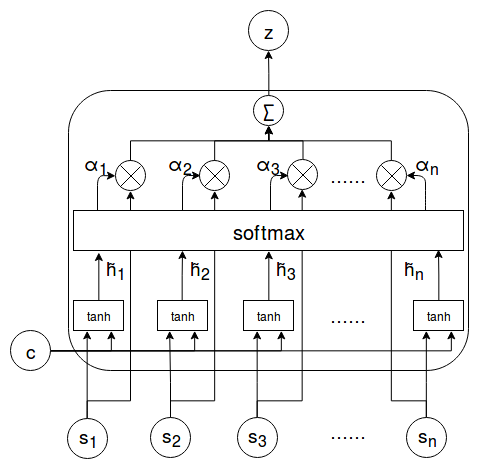
\includegraphics[width=2.8in]{fig_01.png}
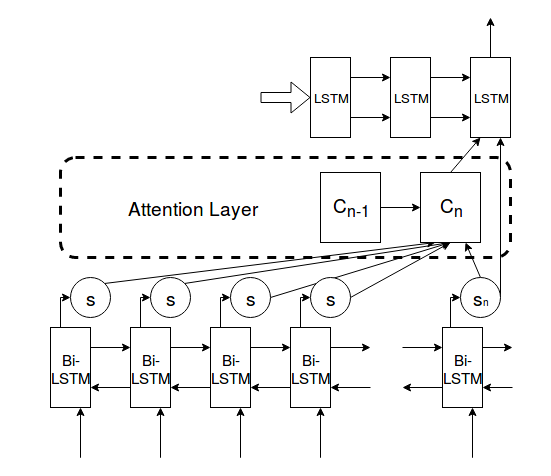
\includegraphics[width=3in]{fig_02.png}
\caption{(Upper) The \textbf{attention layer architecture} employed in the network. At each time step n, this layer computes the attentional hidden state on each previous state and then produces and screened weighted summery of the relevance for each input state according to the context vector}
\caption{(Lower) The \textbf{whole Attention-based network} propsoed in this paper.}. 
\end{figure}


\section{Experiment}
\subsection{Material}
In sleep stage classification study, researchers tipycally use polysomnographic (PSG) recorded data as the diagnostic material \cite{prabhavalkar2017analysis}. The PSG recording experiments are usually conducted in a hospital or sleep center with biological signals such as electroencephalogram (EEG), electrooculogram (EOG), electrocardiogram (ECG) and electromyogram (EMG) of a patient being recorded simulatenously during a whole night experiment \cite{ronzhina2012sleep}.

After the data collection procedures, these signals will be split into epochs with 30 seconds. In clinical practice, the classfication for stages of sleep mainly depends on visual observations on epochs according to standards and terminologies established by Rechtschaffen and Kales (R\&K) sleep scoring manual \cite{rechtschaffen1968manual}, or the manual of American Academy of Sleep Medicine (AASM) \cite{berry2012aasm}.

\begin{table}[!t]
% increase table row spacing, adjust to taste
\renewcommand{\arraystretch}{1.3}
\caption{Description of the train and test set for each fold with respect to each sleep stage after removing noisy epochs (Number of epochs and Ratio[\%]}
\centering
\begin{tabular}{lccccl}
\toprule
  & W & N1 & N2 & N3 & R\\
\midrule
 Number & 5833 & 4248 & 8611 & 3538 & 3206 \\
 Ratio(\%) & 22.9 & 16.7 & 33.9 & 13.9 & 12.6 \\ 
\end{tabular}
\end{table}

In this investigation, we introduced a dataset contains PSGs of overnight record with 512 Hz of sampling rate recorded from 28 Asian female and male adults. According to recently proposed research \cite{chambon2017deep}, there is a trade-off for classification performance among the number of channels, the number of records and spatial extension. The PSG data we investigated includes 6 EEGs, 2 EOG, 4 EMGs 1 ECG and the snore signal. The labels were tagged by several experienced experts according to the AASM guidebook with 5 labels, Awake (W), NREM-1 (N1), NREM-2 (N2), NREM-3 (N3) and REM (R). We firstly separated the records into 30-second long epochs combined with label, excluded the epochs labeled by "?" and then concatenated them into two type of set: one was mixed with respect to epochs, the other was mixed with respect to subjects. Thus we have to kind of dataset, one has 25436 epochs as example shown in Table I; the other has 28 examples with 900 to 1000 epochs. Details about the dataset is attached on the appendix. In this paper, we test
The model was tained to minimize the categorical crossentropy with a balanced loss function in order to obtain a relatively impartiality model prediction for all of the sleep stage. What is more, for the purpose of enchancing the discrimination of the normaly under-represented stage, like N1, we increased its weight in the loss function. To test our model, we trained the model with 5-fold cross-validation (CV) with the two datasets respectively for its abilities of learning representations for each sleep stage and the generalization among different people. The model was implemented in \emph{Keras} with a \emph{Tensorflow} backend. As an extension, we also evaluate the classifier's performance with multiple values of class, i.e. $C = 2\ to\ 6$, as our model on both of these two dataset and it all achieve performs of the state-of-the-art methods.

\subsection{Preprocessing}
In preprocessing procedure, we filter the EEG signals into five frequency band, alpha, delta, theta, beta and gamma according to previous studies and the AASM manual \cite{ronzhina2012sleep,ebrahimi2008automatic,berry2012aasm}. Then the signals are combined together again to produce a new single signal with the shape of $(-1, 512\times30)$. The '-1' denotes the number of the epochs in each sample.
\subsection{Feature extraction}
In this experiment, we trained our models on the features extracted from original PSG data records: time domain and frequency domain features mentioned in previous proposed papers \cite{ronzhina2012sleep,ebrahimi2008automatic,chapotot2010automated}.

Specifically, we firstly caculated the power spectral density as the energy of the 5 frequency band for each channel: delta ($\delta$, 1 - 4 Hz), theta ($\theta$, 4 - 8 Hz), alpha ($\alpha$, 8 - 14 Hz), beta ($\beta$ 14 - 31 Hz), gamma ($\gamma$, 31 - 50 Hz). The ratio (PSD of each band to PSD of the whole) and the relative value (PSD of each band to another band) are also extracted from the PSD result. What is more, the statistic values such as maximum, minimum, mean, standard deviation, skewness and kurtosis are calculated from both the time and frequency domain. Furthermore, the Hjorth features, 95\% and 50\% of spectral edge frequency and the statistics of them are included as suppplementary features. Finally the feature set contains 770 features with 30 time-step (one second for each without overlap).

Since some of the sleep stages' definition and classification contains the stages of the previous epochs, we included features from 2 epochs before and after the current epoch respectively ($30\times 2$ seconds for both side) \cite{chambon2017deep}.
\subsection{Training}
In the experiments, we used one single machine with Intel E5-2683v2 CPU$\times$2, and 128GB memory, equiped with a Nvidia GeForce GTX 1080 graphics card. We used the recorded data and the devision of dataset as mentioned in $Subsection\ A$. 

The model was tained to minimize the categorical crossentropy with a balanced loss function in order to obtain a relatively impartiality model prediction for all of the sleep stage. What is more, for the purpose of enchancing the discrimination of the normaly under-represented stage, like N1, we increased its weight in the loss function. To test our model, we trained the model with 5-fold cross-validation (CV) with the two datasets respectively for its abilities of learning representations for each sleep stage and the generalization among different people. The model was implemented in \emph{Keras} with a \emph{Tensorflow} backend. As an extension, we also evaluate the classifier's performance with multiple values of class, i.e. $C = 2\ to\ 6$, as other previous research \cite{nakamura2017complexity}. As a comparison, we employed an Gradient Boosting Classifier implemented with \emph{XGBoost} \cite{Chen2016XGBoost} and a 2-layer LSTM network training on the same data.


\section{Conclusion}
The conclusion goes here.





% if have a single appendix:
%\appendix[Proof of the Zonklar Equations]
% or
%\appendix  % for no appendix heading
% do not use \section anymore after \appendix, only \section*
% is possibly needed

% use appendices with more than one appendix
% then use \section to start each appendix
% you must declare a \section before using any
% \subsection or using \label (\appendices by itself
% starts a section numbered zero.)
%
  

\appendices
\section{Proof of the First Zonklar Equation}
Appendix one text goes here.

% you can choose not to have a title for an appendix
% if you want by leaving the argument blank


The authors would like to thank...


% Can use something like this to put references on a page
% by themselves when using endfloat and the captionsoff option.
\ifCLASSOPTIONcaptionsoff
  \newpage
\fi



% trigger a \newpage just before the given reference
% number - used to balance the columns on the last page
% adjust value as needed - may need to be readjusted if
% the document is modified later
%\IEEEtriggeratref{8}
% The "triggered" command can be changed if desired:
%\IEEEtriggercmd{\enlargethispage{-5in}}

% references section

% can use a bibliography generated by BibTeX as a .bbl file
% BibTeX documentation can be easily obtained at:
% http://mirror.ctan.org/biblio/bibtex/contrib/doc/
% The IEEEtran BibTeX style support page is at:
% http://www.michaelshell.org/tex/ieeetran/bibtex/
\bibliographystyle{IEEEtran}
% argument is your BibTeX string definitions and bibliography database(s)
\bibliography{reference}{}

% that's all folks
\end{document}


